\documentclass[10pt,twocolumn,letterpaper]{article}

\usepackage{acvs}
\usepackage{times}
\usepackage{epsfig}
\usepackage{graphicx}
\usepackage{amsmath}
\usepackage{amssymb}

% Include other packages here, before hyperref.
\usepackage{dsfont}

% If you comment hyperref and then uncomment it, you should delete
% egpaper.aux before re-running latex.  (Or just hit 'q' on the first latex
% run, let it finish, and you should be clear).
\usepackage[pagebackref=true,breaklinks=true,letterpaper=true,colorlinks,bookmarks=false]{hyperref}

\iccvfinalcopy % *** Uncomment this line for the final submission

\def\iccvPaperID{} % *** Enter the Paper ID here
\def\httilde{\mbox{\tt\raisebox{-.5ex}{\symbol{126}}}}

% Pages are numbered in submission mode, and unnumbered in camera-ready
\ificcvfinal\pagestyle{empty}\fi

\begin{document}

%%%%%%%%% TITLE - PLEASE UPDATE
\title{Progressive Distillation for Fast Sampling of Diffusion Models~\cite{progressive} \\ {\rm {\normalsize Minji Kim (minji@snu.ac.kr; 2020-28702), Dept. of Electrical and Computer Engineering, Seoul National University}}}   % **** Enter the paper title and student information here

\maketitle
\thispagestyle{empty}

%%%%%%%%% BODY TEXT - ENTER YOUR RESPONSE BELOW

%%%%%%%%%%%%%%%%%
%%%%%%%%%%%%%%%%%
\section{Introduction}
Despite the effectiveness of diffusion models in generative tasks, the limitation of diffusion models is their slow sampling time.
This paper presents new parameterizations of diffusion models that provide increased stability while using few sample steps.
Specifically, this method distills a trained deterministic sampler using many steps into a new diffusion model that takes half of the original sampling steps.
The proposed distillation procedure does not take more time than it takes to train the original model, and it can generate an image as few as 4 steps, while still maintaining sample quality competitive with state-of-the-art models which requires thousands of diffusion iteration steps.



%%%%%%%%%%%%%%%%%
%%%%%%%%%%%%%%%%%
\section{Progressive Distillation}

\subsection{Overview}
The overview of \textit{Progressive Distillation} is shown in Fig.~\ref{fig:overview}.
The proposed method iteratively halves the number of required sampling steps by distilling a slow teacher diffusion model into a faster student model. The iteration process is as follows:

\begin{enumerate}
    \item Each time the incremental distillation is repeated, the student model is initialized with the copy of the teacher model using the same model parameters and the same model definition.
    \item Sample data from the training set and add noise to the data.
    \item Process the target $\tilde{x}$ by running two DDIM~\cite{ddim} sampling steps based on the teacher model.
    \item Reduce the student step to the half, and set the student model as the new teacher.
\end{enumerate}

The overall algorithm is shown in Fig.~\ref{fig:algorithm}.


% RePaint modifies the standard denoising process in order to condition on the given image content.
% In each step, it samples the known region from the input and the inpainted part from the DDPM output.
% Specifically, given a ground truth image $x$, the unknown pixels $m \odot x$ and the known pixels $(1-m) \odot x$, the known regions in diffusion step $t$, $(1-m) \odot x_t$, could be consistently altered.
% Thus, in each reverse step, $x_{t-1}$ could be obtained by using following equations:
% %
% \begin{equation}
%     x^{known}_{t-1} \sim \mathcal{N}(\sqrt{\bar{\alpha}_t}x_0, (1-\bar{\alpha}_t)\mathbf{I}),
% \end{equation}
% \begin{equation}
%     x^{unknown}_{t-1} \sim \mathcal{N}(\mu_\theta(x_t, t), \Sigma_\theta(x_t, t)),
% \end{equation}
% \begin{equation}
%     x_{t-1} = m \odot x^{known}_{t-1} + (1-m) \odot x^{unknown}_{t-1}.
% \end{equation}
% %
% Thus, $x^{known}_{t-1}$ is sampled using the known pixels in the given image $m \odot x_0$, and $x^{unknown}_{t-1}$ is sampled from the model, given the previous iteration $x_t$ is given.
% Finally, the new sample $x_{t-1}$ is combined using the mask.



%%%%%%%%%%%%%%%%%
%%%%%%%%%%%%%%%%%
\section{Conclusion}

This paper has proposed Progressive Distillation, a method that dramatically reduces the number of sampling steps required to produce high quality images, and potentially other data using diffusion models with deterministic samplers such as DDIM~\cite{ddim}.
To do so, the authors reparameterize the prediction and define stable weight.
By making these models more affordable to run at test time, this work opens a potential that the diffusion model could be applied in environments with time and memory constraints.




\begin{figure}[t]
    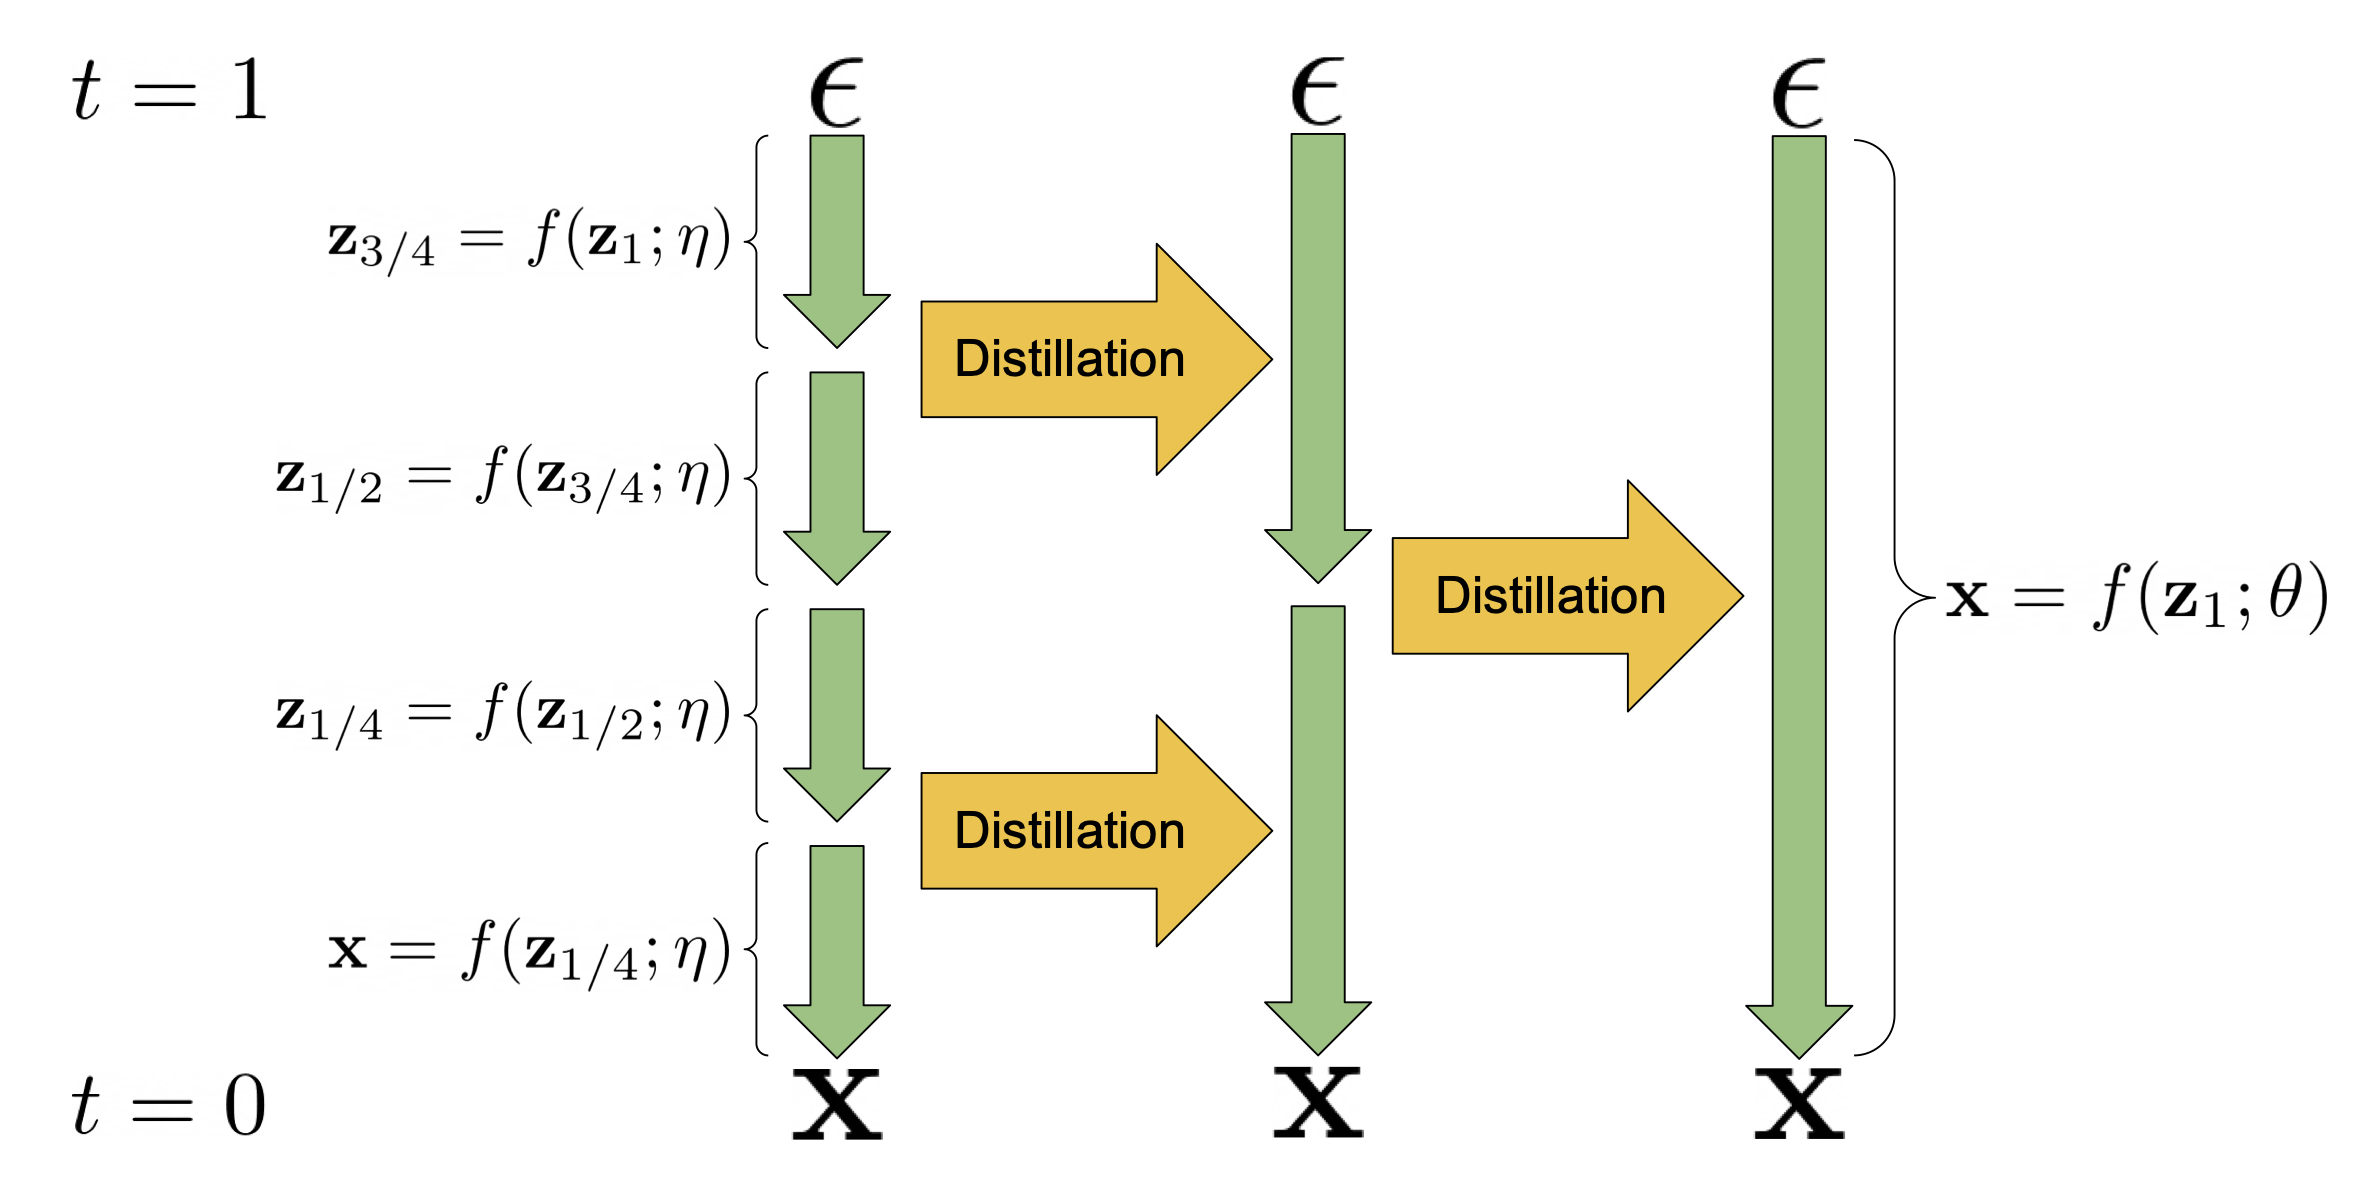
\includegraphics[width=\linewidth]{assets/overview.png}
    \caption{\label{fig:overview}Overview of Progressive Distillation.}
\end{figure}

\begin{figure}[t]
    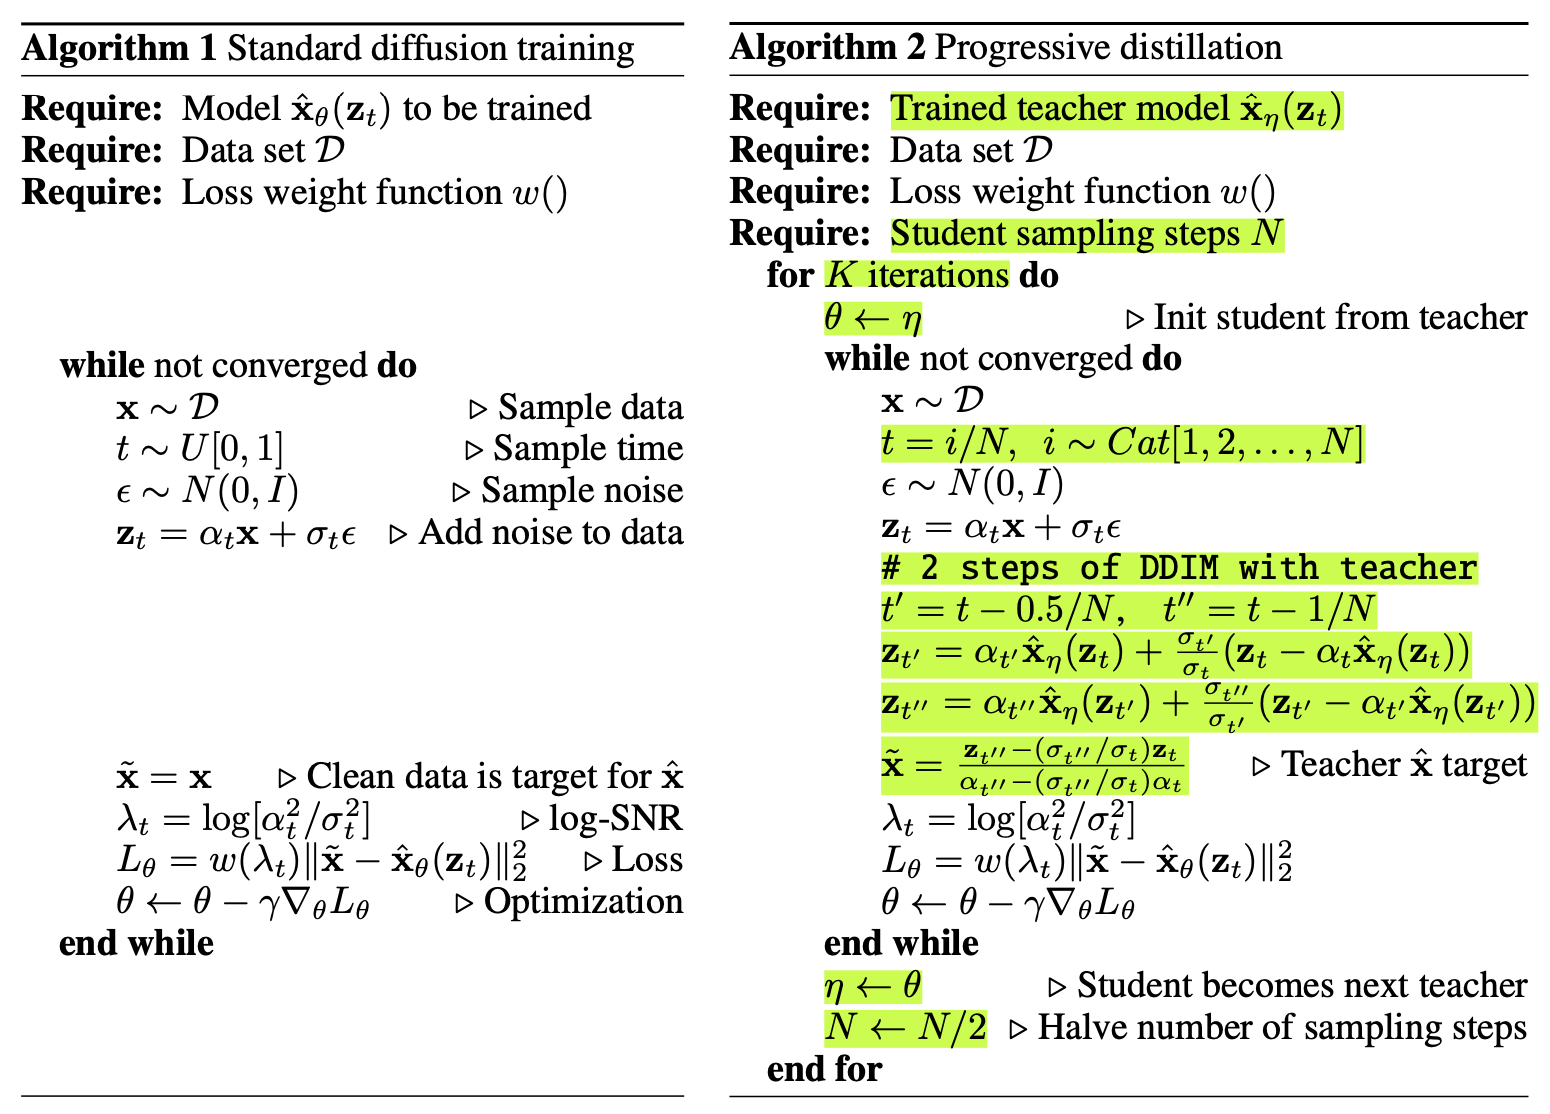
\includegraphics[width=\linewidth]{assets/algorithm.png}
    \caption{\label{fig:algorithm}Algorithm of standard diffusion training and Progressive Distillation.}
\end{figure}



{\small
\bibliographystyle{ieee}
\bibliography{egbib}
}

\end{document}
